V tejto kapitola sa budeme venovať kapitole z knihy Diabetes Technology and Therapeutics\cite{2000}, ktorá ma zaujala kapitolou o inteligentnom diabetickom softvéry.

Pre diabetikov prvého typu je ťažké udržať si stálu alebo optimálnu hladinu cukru \ref{diabetes}. Riešením by bol systém umelej inteligencie pozostávajúci z liečebných algoritmov kalibrovaných prostredníctvom veľkých súborov údajov špecifických pre pacienta.\cite{2000} Znie to zaujímavo, ale chybičku vidím v tom, ako sa ďalej píše v knihe, že je to potrebné spraviť po každej zmene, či už denného režimu, inzulínu alebo športových aktivít. Samotné nastavenie systému nie je v prototype jednoduché a pre množstvo užívateľov neprípustné. 

Softvérový prototyp založený na neurónovej sieti, fuzzy logike a konceptoch expertného systému bol vyvinutý a hodnotený na určenie uskutočniteľnosti a účinnosti predikčného modelu špecifického pre pacienta. Priemerná absolútna percentuálne chyba medzi skutočnými a predpokladanými hodnotami glykémie (hladiny cukru v krvi) zo vstupov denného inzulínu, jedla a informácií o cvičení u testovacích subjektov s Diabetes Melitus 1 bola 10.5 percenta.\cite{2000}
Zdá sa to ako celkom veľká odchýlka, čo aj je, avšak je to stále dosť presné nato, aby to dokázalo zabrániť životu nebezpečným situáciám. 

\subsection{Fuzzy Logika v zdravotníctve}

Typickému zhoršeniu stavu u chorých ľudí predchádzajú rôzne fyziologické zmeny ako pulz alebo krvný tlak. Modifikované upozorňovacie skóre je systém, ktorý bol vyvinutý na assistenciu nemocničnému personálu pri meraní týchto zmien a pri identifikácii pacientov, ktorý potrebujú naliehavú lekársku pomoc aby sa predišlo katastrofálnym stavom. \cite{2019} Systém je aktuálne implementovaný a testovaný v Rashid Center for Diabaetes and Research v UAE.

Primárne požiadavky systému je diaľkový zber vitálnych funkcií pacienta, ktoré sa merajú pomocou snímačov na báze RFID a hodnotenie zdravotného stavu pacienta pomocou algoritmov založených na fuzzy logike\ref{schema}.  Tieto dáta sú následne uchované v elektronických lekárskych záznamoch (EMR) a upozorniť zdravotnícky personál o pacientovom statuse a či potrebuje urgentnú starostlivosť alebo nie. \cite{2019} Následný diagram nám ukazuje schému navrhovaného systému.

\begin{figure}[H]
\centering
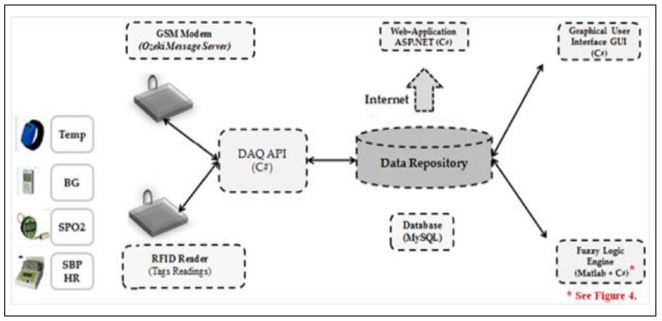
\includegraphics[scale=0.75]{scheme-fuzzy.png}
\caption{Schéma navrhovaného systému \cite{2019}}
\label{schema}
\end{figure}

RFID senzory môžu komunikovať bezdrôtovo s mobilným zariadením a následne pomocou mobilnej siete prenášať informácie do centrálneho monitorovacieho systému - počítača. Tento systém umožňuje implementáciu viacerých užívateľov ako aj počet oblastí monitorovania. \cite{2019} 

Systém pozostáva z rôznych softvérových modulov. Ide o tieto moduly: programovateľné rozhranie pre jednotku zberu dát – aplikácia (DAQ-API), fuzzy logický engine (FLE), databázový manažér (DM), grafické používateľské rozhranie (GUI) a webová aplikácia (Web- Aplikácia). Podrobnosti a funkcie každého softvérového modulu sú zhrnuté nižšie. \cite{2019}

Modul DAQ-API umožňuje interakciu s čítačkou RFID s cieľom zhromažďovať vitálne funkcie pacienta v reálnom čase a zobrazovať ich na obrazovke API. Je to front-end monitorovacie a prevádzkové rozhranie pre používateľov systému.\cite{2019}

DM, GUI a Web-App boli vyvinuté ako echo moduly. Používajú sa na profilovanie používateľov, ukladanie životných funkcií a umožňujú im interakciu so systémom cez web. Podrobný popis týchto echo modulov možno nájsť v štúdii Al-Damour\cite{2013}.\cite{2019}

Model fuzzy logiky má tri postupné procesy: fuzzyfikácia, systém založený na pravidlách a proces defuzzyfikácie.\cite{2019}

\begin{figure}[H]
\centering
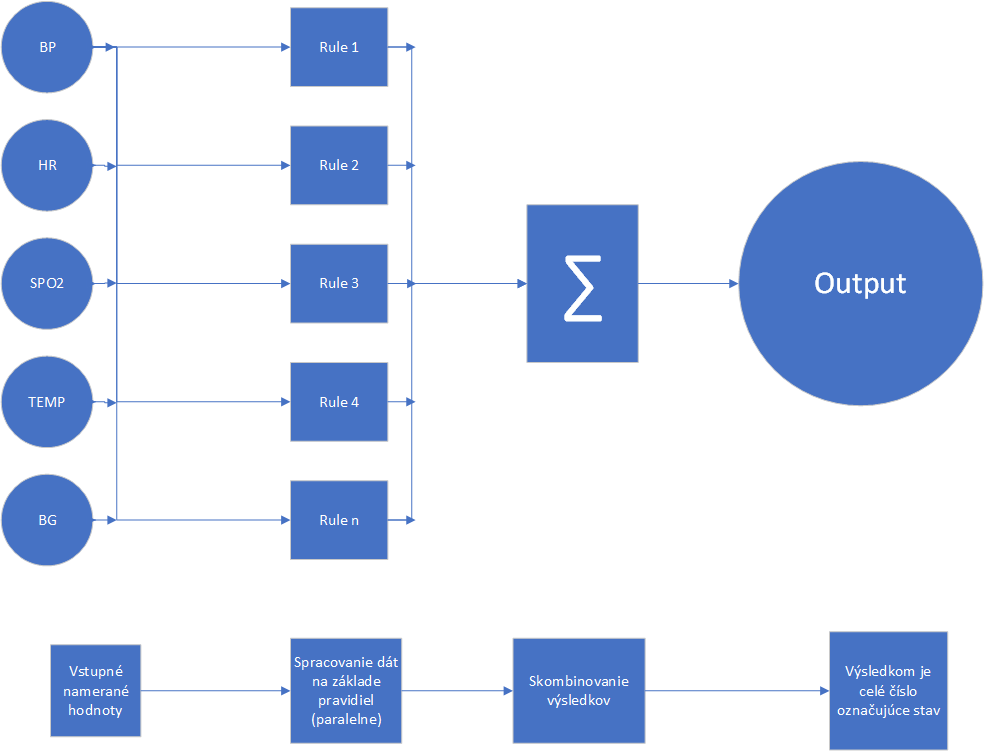
\includegraphics[scale=0.65]{rule-based-engine.png}
\caption{Prekreslená schéma fuzzy procesu podľa článku\cite{2019}}
\label{fuzzy}
\end{figure}

V schéme \ref{fuzzy} vstupujú dáta z RFID senzorov a výsledkom je jedno číslo (status) stavu pacienta. Paralelný charakter pravidiel je jedným z dôležitejších aspektov systémov fuzzy logiky. Namiesto ostrého prepínania medzi režimami na základe bodov prerušenia, logika plynulo prúdi z oblastí, v ktorých správaniu systému dominuje jedno alebo druhé pravidlo. Systém je implementovaný pomocou MATLAB Fuzzy Logic Toolbox. \cite{2019}

\subsection{zhrnutie}
Inteligntné systémy sú riešením avšak s technológiou prichádza aj daň. Systém sa zdá byť na povrchu jednoduchý avšak pre čo najrýchlejšie spracovanie údajov je potreba celkom veľké množstvo výpočtovej techniky a to nerozprávam len o počítačoch na výpočet. Senzory nevydržia dlho. Abbott FreeStyle Libre, čipy, senzory pre kontinuálne sledovanie hladiny cukru, tiež nevydržia večne. A ďalšou požiadavkou bolo pripojenie na mobilnú sieť aby sa dáta dali nahrať na webstránku. Toto je síce menší problém, keďže dáta sa dajú ukladať lokálne a následne naraz odoslať do systému pre spracovanie. Je tam pár háčikov ale blížime sa.